\newpage
\section{Aufgabenstellung 3}

%\subsection{Ausgangssituation}
%Sie sind Teil eines Qualitätssicherungsteams in einem fiktiven Unternehmen, das eine
%E-Commerce-Plattform betreibt. Die Plattform bietet Kameraprodukte an, nutzt KI-gestützte
%Produktsuche, integriert verschiedene Backend-Systeme (z. B. SAP, AWS, NetSuite, HubSpot)
%und führt den Nutzer durch einen komplexen, serviceorientierten Kaufprozess.Ein zentraler
%Bestandteil dieses Systems ist der in der beigefügten Prozessgrafik dargestellte End-to-End-Ablauf,
%vom Website-Besuch bis zur finalen Mail-Bestätigung. Die Architektur umfasst APIs, externe Services,
%Cloud-Provisionierung und ERP-Integration.

%\subsection{Ziel}
%\textit{Erarbeiten Sie als Gruppe eine ganzheitliche Teststrategie für dieses System.
%Die Strategie soll praktikabel sein, typische Herausforderungen im DevOps-Umfeld adressieren
%und die Integration verschiedener Testebenen, Tools und Umgebungen berücksichtigen.}

%\subsection{Bearbeitungsschwerpunkte}
%\textit{Bitte erarbeiten Sie eine Ausarbeitung (max. 6 Seiten + Anhang), in der Sie folgende Punkte behandeln:}

\subsection{Prozessorientierte Teststrategie}
\subsubsection{Prozessübersicht}
Der zentrale Kundenprozess besteht aus folgenden Schritten:
\begin{enumerate}
\item User goes to website
\item Browse for products
\item Add camera to cart
\item Create account
\item Selects shipping
\item Adds photo storage service
\item Completes Checkout
\item Mail confirmation
\end{enumerate}
\subsubsection{Testebenen und -arten}
Für jeden Prozessschritt werden folgende Testebenen angewendet:
\begin{longtable}{|p{3cm}|p{12cm}|}
\hline
\textbf{Testebene} & \textbf{Beschreibung} \\
\hline
Unit-/Component-Tests & Tests einzelner Komponenten und Funktionen, isoliert im Entwicklungsprozess \\
\hline
API-Tests & Prüfung der Schnittstellen zwischen Services und externen Systemen \\
\hline
Integrationstests & Test der Zusammenarbeit von Komponenten und externen Diensten \\
\hline
UI/UX-Tests & Testen der Benutzeroberfläche und Nutzungserfahrung \\
\hline
End-to-End-Tests & Simulation kompletter Benutzerflüsse über alle Prozessschritte hinweg \\
\hline
Performance-Tests & Prüfung des Systemverhaltens unter Last und Stress \\
\hline
Security-Tests & Prüfung auf Sicherheitsprobleme wie XSS, CSRF, etc. \\
\hline
\end{longtable}

\subsubsection{Detaillierte Test-Definition je Prozessschritt}

\paragraph{A. User goes to website \\}
\textbf{Service-Virtualisierung:} GPT-Mock für schnelles Testen, simulierte Userprofile \\
\begin{tabular}{|p{3cm}|p{12cm}|} 
\hline
\textbf{Testarten} & \textbf{Testfokus} \\
\hline
Unit/Component & Performance der Startseiten-Komponenten, Responsive Design, Werbeelemente \\
\hline
API & GPT-Integration für personalisierte Empfehlungen, Content-API-Abrufe \\
\hline
Nicht-funktional & XSS-Vulnerabilities, Content Security Policy, Ladezeit unter 2 Sekunden, WCAG 2.1 AA-Konformität \\
\hline
\end{tabular}


\paragraph{B. Browse for products\\}
\textbf{Service-Virtualisierung:} GPT-Mock für Produktempfehlungen, simulierte Produktkatalog-API \\
\begin{tabular}{|p{3cm}|p{12cm}|}
\hline
\textbf{Testarten} & \textbf{Testfokus} \\
\hline
Unit/Component & Filterkomponenten-Verhalten, Suchfunktionalität, Produktkatalog-Darstellung \\
\hline
API & Produkt-API-Antwortzeiten und -struktur, Suchoptimierung und -relevanz \\
\hline
Nicht-funktional & Reaktionszeit der Suche < 0.5 Sekunden, Verhalten bei gleichzeitiger Suche von 1000+ Nutzern \\
\hline
\end{tabular}


\paragraph{C. Add camera to cart \\}
\textbf{Service-Virtualisierung:} SAP-Mock für Verfügbarkeitsprüfungen, simulierte Verzögerungen \\
\begin{tabular}{|p{3cm}|p{12cm}|}
\hline
\textbf{Testarten} & \textbf{Testfokus} \\
\hline
Unit & Warenkorb-Komponente, Preisberechnung \\
\hline
Integration & SAP-Anbindung zur Verfügbarkeitsprüfung \\
\hline
API & Warenkorb-API, SAP-API für Lagerbestandsprüfung \\
\hline
Nicht-funktional & Reaktionszeit der Warenkorb-Operationen, Konsistenz bei gleichzeitigen Zugriffen \\
\hline
\end{tabular}


\paragraph{D. Create account\\}
\textbf{Service-Virtualisierung:} NetSuite-Mock für Account-Erstellung, HubSpot-Mock\\
\begin{tabular}{|p{3cm}|p{12cm}|}
\hline
\textbf{Testarten} & \textbf{Testfokus} \\
\hline
Unit & Registrierungsformular, Validierungslogik \\
\hline
Integration & NetSuite-Account-Erstellung, HubSpot-Anbindung \\
\hline
API & Account-Erstellungs-API, Authentifizierungs-Workflows \\
\hline
Nicht-funktional & Passwort-Policies, Account-Übernahme-Schutz, DSGVO-Konformität \\
\hline
\end{tabular}


\paragraph{E. Selects shipping \\}
\textbf{Service-Virtualisierung:} SAP-Mock für Versandverifizierung, Simulation internationaler Versandoptionen \\

\begin{tabular}{|p{3cm}|p{12cm}|}
\hline
\textbf{Testarten} & \textbf{Testfokus} \\
\hline
Unit & Versandoptionen-Komponenten \\
\hline
Integration & SAP-Integration für Versandoptionen \\
\hline
API & Versandkosten-Berechnung-API, Lieferzeit-Prognose-API \\
\hline
Nicht-funktional & Reaktionszeiten, korrekte Versandoptionen bei verschiedenen Ländercodes \\
\hline
\end{tabular}

\paragraph{F. Adds photo storage service\\}
\textbf{Service-Virtualisierung:} AWS-Service-Mock für Provisioning-Simulation \\
\begin{tabular}{|p{3cm}|p{12cm}|}
\hline
\textbf{Testarten} & \textbf{Testfokus} \\
\hline
Unit & Storage-Plan-Auswahl-Komponenten \\
\hline
Integration & AWS-Service-Provisioning \\
\hline
API & Storage-Service-API-Aufrufe, Pricing-API für additive Services \\
\hline
Nicht-funktional & Service-Aktivierungszeiten, Fehlerbehandlung bei AWS-Provisioning-Problemen \\
\hline
\end{tabular}


\paragraph{G. Completes Checkout\\}
\textbf{Service-Virtualisierung:} Payment-Service-Mock, NetSuite-Mock für Order-Updates \\

\begin{tabular}{|p{3cm}|p{12cm}|}
\hline
\textbf{Testarten} & \textbf{Testfokus} \\
\hline
Unit & Bezahlprozess-Komponenten, Zusammenfassung \\
\hline
Integration & Integration mit NetSuite für Bestellaktualisierung \\
\hline
API & Checkout-API, Zahlungsverarbeitungs-API \\
\hline
Nicht-funktional & PCI-DSS-Konformität, Zahlungssicherheit, Performance, Transaktions-Rollback \\
\hline
\end{tabular}

\newpage

\paragraph{H. Mail confirmation\\}
\textbf{Service-Virtualisierung:} E-Mail-Service-Mock für Zustellungssimulation\\

\begin{tabular}{|p{3cm}|p{12cm}|}
\hline
\textbf{Testarten} & \textbf{Testfokus} \\
\hline
Unit & E-Mail-Template-Rendering \\
\hline
Integration & E-Mail-Versandsystem-Integration \\
\hline
API & E-Mail-API-Aufrufe, Bestätigungs-Tracking-API \\
\hline
Nicht-funktional & E-Mail-Zustellung-Rate $>$ 99,5\%, E-Mail-Versandzeit $<$ 30 Sekunden \\
\hline
\end{tabular}

\subsection{End-to-End-Testszenarien}
\subsubsection{Hauptszenarien}
\paragraph{Standardablauf: Kompletter Kaufprozess}
\begin{itemize}
\item \textbf{Beschreibung:} Vollständiger Durchlauf vom Website-Besuch bis zur E-Mail-Bestätigung
\item \textbf{Testdaten:} Neuer Benutzer, verfügbares Kameraprodukt, Standard-Versand, Basic-Speicherpaket
\item \textbf{Erwartetes Ergebnis:} Erfolgreicher Kaufabschluss, korrekte Bestellbestätigung per E-Mail
\item \textbf{Automatisierungsgrad:} 90\% automatisiert (Playwright/Cypress)
\item \textbf{Testumgebung:} Staging mit teilweise virtualisierten Services
\end{itemize}
\paragraph{Szenario: Rückkehrender Kunde mit Login}
\begin{itemize}
\item \textbf{Beschreibung:} Login eines Bestandskunden und Durchführung eines Kaufs mit gespeicherter Adresse
\item \textbf{Testdaten:} Existierender Account, Produktvariante mit Zubehör, vorhandener Fotospeicher
\item \textbf{Erwartetes Ergebnis:} Korrekte Nutzung gespeicherter Daten, erfolgreicher Checkout
\item \textbf{Automatisierungsgrad:} 85\% automatisiert
\item \textbf{Testumgebung:} Staging mit Echtanbindung an HubSpot
\end{itemize}
\paragraph{Szenario: Foto-Kursbuchung}
\begin{itemize}
\item \textbf{Beschreibung:} Buchung eines Fotografie-Kurses statt eines physischen Produkts
\item \textbf{Testdaten:} Neuer Benutzer, Online-Kurs "DSLR-Fotografie für Einsteiger"
\item \textbf{Erwartetes Ergebnis:} Erfolgreiche Kursbuchung, Aktivierungslink in der E-Mail
\item \textbf{Automatisierungsgrad:} 80\% automatisiert
\item \textbf{Testumgebung:} Staging mit AWS-Integration
\end{itemize}
\subsubsection{Fehlerszenario-Tests}
\paragraph{Produkt während Checkout nicht mehr verfügbar}
\begin{itemize}
\item \textbf{Beschreibung:} Simulation eines Lagerbestandsproblems während des Checkouts
\item \textbf{Testdaten:} Produkt mit kritischem Lagerbestand, der während des Prozesses auf 0 sinkt
\item \textbf{Erwartetes Ergebnis:} Nutzerfreundliche Fehlerbehandlung, alternative Produktvorschläge
\item \textbf{Automatisierungsgrad:} 70\% automatisiert, 30\% manuelle Validierung
\item \textbf{Testumgebung:} Staging mit manipuliertem SAP-Mock
\end{itemize}
\paragraph{Zahlungsabbruch und Wiederaufnahme}
\begin{itemize}
\item \textbf{Beschreibung:} Test der Wiederaufnahme eines unterbrochenen Zahlungsprozesses
\item \textbf{Testdaten:} Bestandskunde mit vollständigem Warenkorb, Zahlungsabbruch
\item \textbf{Erwartetes Ergebnis:} Persistenz des Warenkorbs, erfolgreiche Wiederaufnahme, Benachrichtigung
\item \textbf{Automatisierungsgrad:} 65\% automatisiert
\item \textbf{Testumgebung:} Staging mit Payment-Service-Mock
\end{itemize}
\paragraph{AWS-Service-Aktivierungsfehler}
\begin{itemize}
\item \textbf{Beschreibung:} Test des Fehlerverhaltens bei AWS-Provisioning-Problemen
\item \textbf{Testdaten:} Erfolgreich abgeschlossene Bestellung mit Fotospeicherdienst
\item \textbf{Erwartetes Ergebnis:} Fehlerbenachrichtigung, automatisierter Wiederholungsversuch, Support-Ticket
\item \textbf{Automatisierungsgrad:} 75\% automatisiert
\item \textbf{Testumgebung:} Staging mit fehlersimulierendem AWS-Mock
\end{itemize}


\subsection{Testumgebungsstabilisierung}
%\begin{itemize}
%    \item \textit{Wie stellen Sie in der Entwicklungs- und Integrationsphase eine stabile
%Testumgebung sicher, insbesondere angesichts externer Systeme (SAP, AWS, GPT, HubSpot etc.)?}
%    \item \textit{Wie kann Service-Virtualisierung oder Mocking zum Einsatz kommen?}
%    \item \textit{Welche Datenanforderungen bestehen (z. B. synthetische Testdaten, Daten-Maskierung)?}
%\end{itemize}

Für unsere E-Commerce-Plattform mit ihren vielfältigen Integrationen (SAP, AWS, GPT, HubSpot) setzen wir auf:

\begin{itemize}
    \item \textbf{Infrastruktur als Code (IaC):} Wir nutzen Terraform/CloudFormation, um isolierte
    Testumgebungen automatisiert zu erstellen und zu verwalten.
    \item \textbf{Umgebungsmodellierung:} Jede Testumgebung wird für bessere Transparenz und
    Kontrolle mit ihren Komponenten, Konfigurationen und Testdaten dokumentiert.
    \item \textbf{Containerisierung:} Kubernetes-Namespaces für kurzlebige, isolierte Testumgebungen.
    \item \textbf{Sandbox-Accounts:} Dedizierte Test-Accounts für Cloud-Dienste verhindern
    Konflikte zwischen den Teams.
\end{itemize}

Zusammenfassend isolieren und verwalten wir die Infrastruktur mittels IaC
(z.\,B. Terraform/CloudFormation) und nutzen dedizierte Sandbox-Accounts, um Konflikte zu vermeiden.
Service-Virtualisierung ist eine zentrale Strategie die im nächsten Abschnitt beschrieben wird.
Für eine beispielhafte Darstellung der Umgebung siehe Abbildung~\ref{fig:deployment}.

\newpage

\begin{figure}[h!]
    \centering
    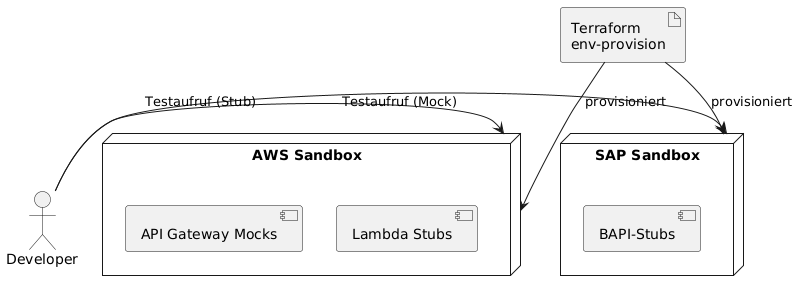
\includegraphics[width=1\textwidth]{fig/stubing.png}
    \caption{Deployment-Diagramm: Virtuelle Testumgebungen via IaC}
    \label{fig:deployment}
\end{figure}

\begin{longtable}{|p{3cm}|p{3cm}|p{3cm}|p{3cm}|p{2cm}|}
\caption{Testumgebungen} \\ \hline    
\hline
\textbf{Umgebung} & \textbf{Hauptzweck} & \textbf{Virtualisierung} & \textbf{Testdaten} & \textbf{Ausführung} \\
\hline
Entwicklung & Entwicklertests, Komponententests & Alle Services virtualisiert & Synthetische Testdaten & Kontinuierlich \\
\hline
CI/CD-Pipeline & Unit/API-Tests, statische Codeanalyse & Alle Services virtualisiert & Synthetische Testdaten & Bei jedem Commit \\
\hline
Integration & Service-Integration, API-Tests & Kritische externe Services virtualisiert & Gemischte Testdaten & Täglich \\
\hline
Staging & E2E-Tests, UAT & Minimale Virtualisierung & Produktionsähnliche Daten & Bei Release-Kandidaten \\
\hline
Produktionsähnlich & Performance, Last, Sicherheit & Keine Virtualisierung & Vollständige Testdaten & Wöchentlich \\
\hline
\end{longtable}

\subsubsection{Service-Virtualisierung und Mock-Ansätze}
Service-Virtualisierung ist entscheidend, wenn externe Systeme nicht verfügbar, instabil oder die
Kosten für die Nutzung für Tests zu hoch sind:

\begin{itemize}
    \item \textbf{REST/HTTP-Interfaces:} WireMock oder Mountebank für die Simulation von REST-APIs
    \cite{wiremock2025}.
    \item \textbf{Cloud-APIs:} AWS LocalStack für lokale Emulation von AWS-Services \cite{aws2021}.
    \item \textbf{ERP-Integration:} Virtualisierung von SAP BAPIs und speziellen Schnittstellen.
    \item \textbf{API-Gateway:} Nutzung von AWS API Gateway zur Erstellung von Mock-Endpunkten.
\end{itemize}

Für abhängige Systeme (ERP oder externe APIs) können Virtualisierungstools realistische
Interaktionen simulieren. Open-Source-Lösungen wie WireMock oder Mountebank
(siehe dazu \citet{byars2018}) stubben REST-/HTTP-Schnittstellen, während Cloud-Tools
(z.\,B. AWS LocalStack) Cloud-APIs lokal emulieren. Der Ablauf ist in Abbildung~\ref{fig:sequence}
dargestellt.

\begin{figure}[h!]
    \centering
    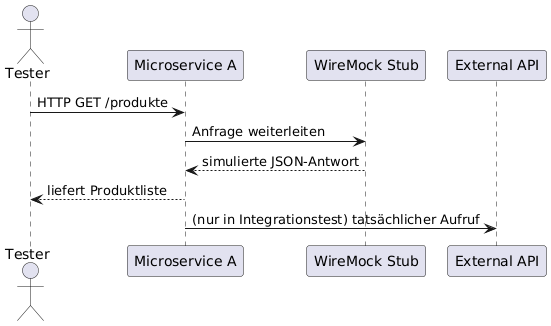
\includegraphics[width=0.8\textwidth]{fig/servicevirti.png}
    \caption{Sequenzdiagramm: Service-Virtualisierung mit WireMock}
    \label{fig:sequence}
\end{figure}

Die Virtualisierung abhängiger Services erfolgt phasengesteuert: Während der Build-Phase kommen
WireMocks zum Einsatz, um Unit- und API-Tests in der Pipeline oder Entwicklungsumgebung zu
unterstützen. In der IaC-Testumgebung emuliert AWS LocalStack Cloud-APIs, um Integrationstests
effizient durchzuführen. Zusätzlich werden SAP-Schnittstellen bereits vor Testbeginn durch Parasoft
Virtualize gestubbt - dies reduziert Latenzen bei der Testvorbereitung und erfüllt Complance-Anforderungen
wie Datenmaskierung. Der gestaffelte Einsatz virtueller Komponenten sichert konsistente Testbedingungen,
unabhängig von externen Systemabhängigkeiten.

\begin{longtable}{|p{2cm}|p{3cm}|p{4cm}|p{2cm}|p{3cm}|}
\caption{Virtualisierungsansatz pro Prozessschritt} \\ \hline
\textbf{System} & \textbf{Prozessschritt} & \textbf{Virtualisierungsansatz} & \textbf{Tool} & \textbf{Umgebung} \\ \hline
\endfirsthead

\multicolumn{5}{c}{\tablename\ \thetable{} -- Fortsetzung} \\ \hline
\textbf{System} & \textbf{Prozessschritt} & \textbf{Virtualisierungsansatz} & \textbf{Tool} & \textbf{Umgebung} \\ \hline
\endhead

GPT & User goes to website & Vortrainierte Antworten für Produktsuche & WireMock & Entwicklung, CI/CD \\ \hline
SAP & Add camera to cart & Statische Verfügbarkeitsantworten & LocalStack & Entwicklung, Integration \\ \hline
SAP & Selects shipping & Konfigurierbare Versandoptionen & WireMock & Integration, Last-Tests \\ \hline
HubSpot & Create account & Service-Provisionierung & Mountebank & Entwicklung, Integration \\ \hline
NetSuite & Create account & Account-Erstellung & WireMock & Alle außer Prod \\ \hline
NetSuite & Completes Checkout & Bestellaktualisierung & WireMock & Integration, Staging \\ \hline
AWS & Adds photo storage & Service-Provisioning & LocalStack & Entwicklung, Integration \\ \hline
\end{longtable}

\subsubsection{Testdatenmanagement}
Um konsistente und compliance-konforme Tests zu gewährleisten, können folgende Ansätze verwendet werden:

\begin{itemize}
    \item \textbf{Datenmaskierung:} Ersetzen von Personally Identifiable Information (PII) mit
    realistischen fiktiven Werten unter Beibehaltung der referentiellen Integrität. \citet{tricentis2024}
    empfiehlt Format-preserving Encryption für PII
    \item \textbf{Synthetische Daten:} Künstliche Datensätze für Spezialfälle und Randszenarien.
    \citet{browserstack2025} kombiniert synthetische und maskierte Daten.
    \item \textbf{Hybridansatz:} Maskierte Produktionsdaten für Basistests, ergänzt durch
    synthetische Daten für Edge-Cases.
    \item \textbf{API-Integration:} CI/CD-Pipeline kann Testdaten über APIs auffrischen,
    zurücksetzen oder klonen.
\end{itemize}

\begin{longtable}{|p{3cm}|p{5cm}|p{3cm}|p{3cm}|}
\caption{Prozessspezifische Testdaten} \\
\hline
\textbf{Prozessschritt} & \textbf{Testdaten-Anforderungen} & \textbf{Quelle} & \textbf{Bereitstellung}\\
\hline
User goes to website & User-Personas, Browser-Profile & Synthetisch & Fixture-Files\\
\hline
Browse for products & Produktkatalog mit Varianten & Prod-Kopie & TDM-Tool (Delphix)\\
\hline
Add camera to cart & Produktvarianten mit Lagerbestandsstufen & Synthetisch & API-Seeding\\
\hline
Create account & Benutzerprofile, E-Mail-Domains & Synthetisch & Faker.js + API\\
\hline
Selects shipping & Verschiedene Länder/Regionen & Prod-Kopie & CSV-Import\\
\hline
Adds photo storage & Storage-Pläne mit Preisen & Aktuelle Konfiguration & Configuration-as-Code\\
\hline
Completes Checkout & Zahlungsmethoden, Gutscheincodes & Synthetisch & API-Seeding\\
\hline
Mail confirmation & E-Mail-Templates, Sprachen & Aktuelle Version & Git-Repository\\
\hline
\end{longtable}

\paragraph{Testdaten-Governance}
Zur Sicherstellung von Datenqualität und Compliance:
\begin{itemize}
\item \textbf{Daten-Klassifizierung:} Kategorisierung von Testdaten nach Sensitivität und Verwendungszweck
\item \textbf{Automatisierte DSGVO-Konformität:} Automatisches Maskieren von personenbezogenen Daten
\item \textbf{Versionsverwaltung:} Testdaten-Snapshots mit Versionierung für Reproduzierbarkeit
\item \textbf{Selbstbedienungsportal:} GUI für Tester zum Anfordern und Verwalten von Testdaten-Sets
\item \textbf{Nutzungsverfolgung:} Logging und Monitoring der Testdatennutzung für Audits
\end{itemize}

\subsection{Testarten und Abdeckung}
\subsubsection{Funktionale Tests}

Zur Abdeckung funktionaler Anforderungen setzen wir folgende Testtypen ein:
\begin{itemize}
    \item \textbf{Unit-Tests:} Für einzelne Module/Services, laufen bei jedem Commit.
    \item \textbf{API-Tests:} Validierung jeder Microservice-Schnittstelle gegen ihre Spezifikation
    (mit JUnit, pytest oder Postman/Newman).
    \item \textbf{Integrationstests:} Testen zusammenhängender Dienste (z.B. Inventarsynchronisation
    von SAP zu NetSuite).
    \item \textbf{End-to-End-Tests:} Simulation realer Benutzerszenarien (Produktsuche, Checkout etc.)
    mit Selenium, Cypress oder Playwright.
\end{itemize}

\subsubsection{Nicht-funktionale Tests}
Zur Prüfung von Performance, Security, Verfügbarkeit und Datenintegrität verwenden wir:

\begin{itemize}
    \item \textbf{Performance/Last-Tests:} Apache JMeter oder Gatling zur Simulation von
    Verkehrsspitzen und Messung der Skalierbarkeit.
    \item \textbf{Security-Tests:} Kombination aus statischer (SAST) und dynamischer (DAST)
    Analyse mit Tools wie SonarQube, Snyk oder OWASP ZAP.
    \item \textbf{Verfügbarkeitstests:} Monitoring der Systemverfügbarkeit unter
    verschiedenen Lastbedingungen.
    \item \textbf{Datenintegritätstests:} Validierung der Datenkonsistenz zwischen SAP,
    NetSuite und AWS.
\end{itemize}

\subsubsection{CI/CD-Pipeline Integration}
Tests sind in der Pipeline wie folgt integriert:

\begin{itemize}
    \item \textbf{Build-Phase:} Unit-Tests (lokal) und API-Tests (gegen Mocks) laufen bei jedem Build.
    \item \textbf{Deployment-Phase:} Integrations- und Smoke-Tests, in IaC-Umgebung nach Deployment
    in Testumgebung (mit SAP/AWS-Virtualisierung).
    \item \textbf{Post-Deployment:} E2E-Tests in Staging-Umgebung (mit SAP/AWS-Virtualisierung).
    \item \textbf{Nachtests:} Performance- und Security-Tests in isolierten Cloud-Sandboxes.
\end{itemize}


\begin{longtable}{|>{\centering\arraybackslash}p{2.5cm}|>{\centering\arraybackslash}p{4cm}|>{\centering\arraybackslash}p{4cm}|>{\centering\arraybackslash}p{3.5cm}|}
\caption{Automatisierungsstrategie pro Prozessschritt} \\
\hline
\textbf{Prozessschritt} & \textbf{Automatisierungsgrad} & \textbf{Frameworks} & \textbf{CI/CD-Integration} \\
\hline
User goes to website & 90\% & Jest, Lighthouse & Commit-Stage \\
\hline
Browse for products & 85\% & TestCafe, Cypress & Täglich \\
\hline
Add camera to cart & 90\% & Cypress, API-Tests & Commit-Stage \\
\hline
Create account & 80\% & Playwright, API-Tests & Täglich \\
\hline
Selects shipping & 85\% & Cypress, API-Tests & Täglich \\
\hline
Adds photo storage & 75\% & Selenium, API-Tests & Täglich \\
\hline
Completes Checkout & 70\% & Cypress, API-Tests & Release-Gate \\
\hline
Mail confirmation & 95\% & API-Tests, E-Mail-Tests & Release-Gate \\
\hline
\end{longtable}

\subsubsection{Testausführungsorte}
Die Tests werden an verschiedenen Ausführungsorten ausgeführt:

\begin{table}[h!]
\centering
\caption{Testausführungsorte und virtualisierte Services}
\label{tab:testorte}
\begin{tabular}{p{3.5cm}p{4cm}p{5cm}}
\toprule
\textbf{Testtyp} & \textbf{Ausführungsort} & \textbf{Virtualisierte Services} \\
\midrule
Unit-Tests & Lokale Entwicklerumgebung / Build-Pipeline & 
 WireMock (externe APIs)
 Lokale DB-Clones \\
API-/Integrationstests & IaC-basierte Testumgebung (AWS Sandbox) & 
  AWS LocalStack (Cloud-Services)
  SAP-Mocks \\
End-to-End-Tests & Staging-Umgebung (Kubernetes-Namespace) & 
  HubSpot-\& GPT-Virtualisierung 
  via API Gateway \\
Performance/Security & Dedizierte Lastumgebung (BlazeMeter/k6 Cloud) & 
Vollständig isolierte Sandbox-Accounts \\
\bottomrule
\end{tabular}
\end{table}

\subsection{Testeffizienz und Wartbarkeit}
%\begin{itemize}
%    \item Wie strukturieren Sie Tests, um gezielt auf Systemveränderungen (z. B. SAP-Upgrade)
%reagieren zu können?
%    \item Wie nutzen Sie z. B. Impact Analysis, modulare Architekturen oder risikobasiertes Testen,
%um Wiederverwendbarkeit und Selektivität zu ermöglichen?
%\end{itemize}
\subsubsection{Strukturierung der Tests für Systemveränderungen}
Um flexibel auf Änderungen (wie SAP-Upgrades oder Microservice-Updates) reagieren zu können:

\begin{itemize}
    \item \textbf{Modulare Testarchitektur:} Tests sind nach Komponenten (Unit), Systemen (Integration)
    und E2E-Prozessen organisiert, um Änderungen in SAP oder Microservices isoliert zu validieren
    \item \textbf{Shared Libraries:} Gemeinsame Funktionen und Daten-Fixtures vermeiden Duplikationen.
    \item \textbf{Page Object Model:} Kapselung von UI-Interaktionen für bessere Wartbarkeit.
    \item \textbf{API-Client-Bibliotheken:} Wiederverwendbare Clients für API-Tests.
\end{itemize}

\subsubsection{Effizienzansätze}
Zur Optimierung des Testaufwands setzen wir ein:

\begin{itemize}
    \item \textbf{Impact Analysis:} Identifikation relevanter Tests nach Code-Änderungen durch
    Version-Control-Hooks und spezielle Tools.
    \item \textbf{Risikobasiertes Testen:} Priorisierung von Features mit hoher Geschäftsrelevanz
    oder bekannter Komplexität.
    \item \textbf{Sprint-basierte Testplanung:} QA und Entwicklung bewerten gemeinsam
    Änderungsauswirkungen und passen Testpläne an.
\end{itemize}

\subsection{Reporting \& Testtransparenz}

\subsubsection{Dokumentation und Auswertung}
Für transparentes Reporting nutzen wir:

\begin{itemize}
    \item \textbf{CI/CD-Dashboard:} Unit- und Integrationstestergebnisse
    (Pass/Fail, detaillierte Logs) im CI-Dashboard.
    \item \textbf{Coverage-Reports:} JaCoCo, Coverage.py für Codeabdeckungsanalysen.
    \item \textbf{Test-Framework-Reports:} HTML/XML-Reports von Frameworks wie pytest, TestNG
    oder Cucumber.
    \item \textbf{Aggregationstools:} Allure oder ReportPortal für umfassendere Analysen.
    \item \textbf{Monitoring-Dashboards} Grafana/Kibana zur Visualisierung von Performance-Metriken.
\end{itemize}

\subsubsection{Stakeholder-spezifische Sichten}

\begin{itemize}
    \item \textbf{Entwickler:Innen:} Detaillierte Fehlerprotokolle und Stack-Traces zur schnellen
    Fehlerbehebung.
    \item \textbf{QA-Leads und Team:} Übersichts-Dashboards mit Testfallstatus, Defect-Counts und
    Coverage (z.B. in TestRail, Xray oder Zephyr).
    \item \textbf{Operations:} Monitoring-Tools (CloudWatch, Prometheus/Grafana) für Performance
    und Systemgesundheit.
    \item \textbf{Management:} Hochrangige Indikatoren wie Testbestehensraten, Coverage-Prozentsätze
    und Business-Risikobewertungen.
    \item \textbf{DevOps-Metriken:} DORA-Metriken (Deployment-Frequenz, Change-Failure-Rate) neben
    Testmetriken.
\end{itemize}

Durch automatisierte Berichterstellung (per E-Mail, Slack oder interne Dashboards) stellen wir
Rechenschaftspflicht und zeitnahes Feedback sicher.
%\begin{itemize}
%    \item Wo und wie sollen Testergebnisse dokumentiert und ausgewertet werden
%(z. B. Dashboards, Logs, automatisierte Reports)?
%    \item Wer sind die Stakeholder für das Reporting (Dev, QA, Ops, Management)?
%\end{itemize}

Diese Strategien ermöglichen eine schlanke, aber effektive Testsuite, die sich an verändernde
Anforderungen anpasst und gleichzeitig den Wartungsaufwand kontrolliert.

\subsection{Toolauswahl und Integration}
\subsubsection{Testautomatisierung}

\begin{itemize}
    \item \textbf{UI-Tests:}  Selenium WebDriver oder Playwright für browserübergreifende Tests
    \item \textbf{Unit/Integration:} JUnit/TestNG oder pytest
    \item \textbf{BDD:} Cucumber oder Behave
    \item \textbf{API-Testing:} Postman/Newman oder REST-assured
    \item \textbf{Cloud-Testing:} LambdaTest für Tests auf verschiedenen OS/Browser-Kombinationen
\end{itemize}

\subsubsection{Performance-Testing}
\begin{itemize}
    \item \textbf{Protokollebene:} Apache JMeter für verteilte Lasttests
    \item \textbf{Code-basiert:} Gatling für programmierbare Lastszenarien
    \item \textbf{Cloud-Services:} BlazeMeter, k6 Cloud für On-Demand-Skalierung
\end{itemize}

\subsubsection{Service-Virtualisierung}
\begin{itemize}
    \item \textbf{HTTP-Stubbing:} WireMock oder Mountebank
    \item \textbf{Cloud-API-Emulation:} AWS API Gateway Mocks, LocalStack
    \item \textbf{Enterprise-Protokolle:} Parasoft Virtualize, Tricentis StubWeb für komplexe
    Unternehmensschnittstellen
\end{itemize}

\subsubsection{Testdatenmanagement}
\begin{itemize}
    \item \textbf{Enterprise-Plattformen:} Informatica, Delphix oder open source Lösungen wie
    Data Masker
    \item \textbf{Datengenerierung:} Faker-Bibliotheken wie Mockaroo, dbForge Data Generator
    \item \textbf{Datenbank-Cloning:} Dockerisierte Test-DBs für isolierte Testdatenbanken
\end{itemize}

\subsubsection{Reporting \& Testmanagement}
\begin{itemize}
    \item \textbf{Orchestrierung:} GitLab CI oder Jenkins für CI/CD-Pipelines
    \item \textbf{Reporting:} Allure, ReportPortal oder Grafana/Kibana für Dashboards
    \item \textbf{Code-Qualität:} SonarQube für statische Code-Analyse
    \item \textbf{Testmanagement:} TestRail, Xray oder Zephyr für Testfallmanagement
    \item \textbf{Monitoring:} Prometheus/Grafana für Performance- und Verfügbarkeitsüberwachung
\end{itemize}

Alle gewählten Tools unterstützen DevOps-Praktiken: Sie integrieren sich in CI/CD-Pipelines,
bieten REST-APIs oder Plugins und skalieren in der Cloud.

\subsection{Zusammenfassung}
Unsere Teststrategie für die E-Commerce-Plattform stellt durch ein umfassendes Konzept sicher,
dass alle funktionalen und nicht-funktionalen Anforderungen effektiv getestet werden.
Wir setzen auf stabile, automatisierte Testumgebungen, Service-Virtualisierung für externe Systeme
und ein effizientes Testdatenmanagement. Die Integration verschiedener Testarten in die
CI/CD-Pipeline, verbunden mit einer modularen, wartbaren Testarchitektur und transparentem
Reporting, garantiert kontinuierliches Qualitätsfeedback und hält mit agilen Lieferanforderungen
Schritt.

\newpage
\subsection{Anhang}
\subsubsection{Tool-Landschaft Überblick}
\begin{longtable}{|p{3.5cm}|p{3.5cm}|p{4cm}|p{3cm}|}
\caption{Tool-Landschaft Überblick mit Testebenen} \\ \hline
\textbf{Kategorie} & \textbf{Tools} & \textbf{Anwendungsbereich} & \textbf{Testebene} \\ \hline
\endfirsthead

\multicolumn{4}{c}{\tablename\ \thetable{} -- Fortsetzung} \\ \hline
\textbf{Kategorie} & \textbf{Tools} & \textbf{Anwendungsbereich} & \textbf{Testebene} \\ \hline
\endhead

Testautomatisierung &
Selenium, Playwright, Cypress, JUnit/TestNG, pytest, Cucumber, Postman/Newman &
UI- und Funktionstest, API-Test &
Unit/Component, System, E2E \\ \hline

Performance-Testing &
Apache JMeter, Gatling, k6, BlazeMeter &
Last- und Performance-Tests &
System, End-to-End \\ \hline

Service-Virtualisierung &
WireMock, Mountebank, AWS LocalStack, API Gateway Mocks, Parasoft Virtualize &
Mock-Services für APIs und Systeme &
Build-Phase, Integrationstests \\ \hline

Testdatenmanagement &
Delphix, Informatica TDM, Redgate Data Generator, Faker-Bibliotheken &
Datenmaskierung, Synthetische Daten &
Alle Testebenen, Pipeline-übergreifend \\ \hline

Reporting \& Testmanagement &
Jenkins/GitLab CI, Allure Report, ReportPortal, Xray/Zephyr/TestRail, Grafana/ELK &
Testdokumentation, Auswertung &
Pipeline-übergreifend, Stakeholder-Dashboards \\ \hline

\end{longtable}

Ein Beispiel für eine für eine wissenschaftliches Paper das Tools vergleicht ist Software Testing:
5th Comparative Evaluation: {Test-Comp 2023} von \cite{beyer2023}

\subsubsection{Testarchitektur und Komponentendiagramm}

\begin{figure}[h!]
    \centering
    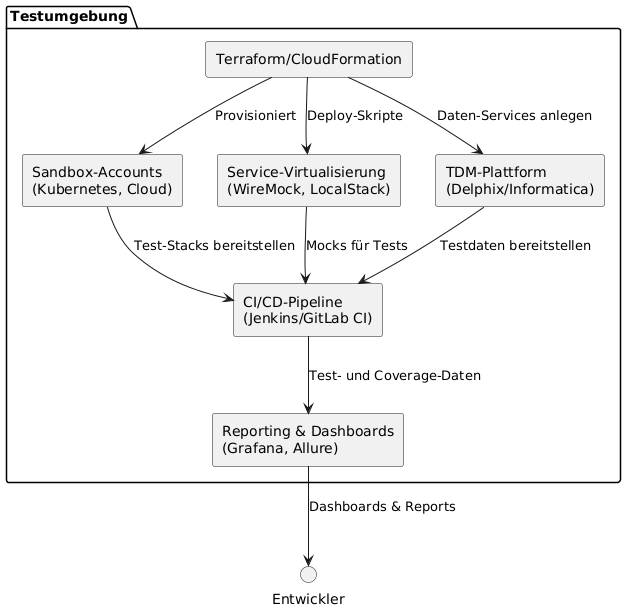
\includegraphics[width=0.8\textwidth]{fig/test_architecture_enviroment.png}
    \caption{Architektur: Komponentenübersicht der Testumgebung}
    \label{fig:architecture}
\end{figure} 

In Abbildung \ref{fig:architecture} ist unsere Testarchitektur dargestellt.
Diese Architektur zeigt die verschiedenen Komponenten, die in der Testumgebung verwendet werden,
einschließlich der Testautomatisierung, Service-Virtualisierung und Testdatenmanagement-Tools.
Die Architektur ist so gestaltet, dass sie eine klare Trennung zwischen den verschiedenen Schichten
der Testumgebung ermöglicht und gleichzeitig eine einfache Integration in die CI/CD-Pipeline
gewährleistet.

\begin{itemize}
    \item \textbf{IaC}  (Terraform/CloudFormation) stellt Sandbox-Accounts, Virtualisierungs-
    und TDM-Komponenten bereit.
    \item \textbf{Service-Virtualisierung} (WireMock, LocalStack) simuliert externe Systeme und
    liefern damit isolierte Umgebungen und Mock-Services.
    \item \textbf{TDM} versorgt die Pipeline mit maskierten oder synthetischen Daten.
    \item \textbf{CI/CD-Pipeline} (Selenium, JUnit, Postman) orchestriert Tests und stellt
    Ergebnisse ins Reporting.
    \item \textbf{Reporting} (Allure, Grafana) aggregiert Testergebnisse und stellt sie in
    Dashboards dar.
\end{itemize}

\subsubsection{Ablaufflow der Continuous-Testing-Pipeline}

\begin{figure}[h!]
\centering
    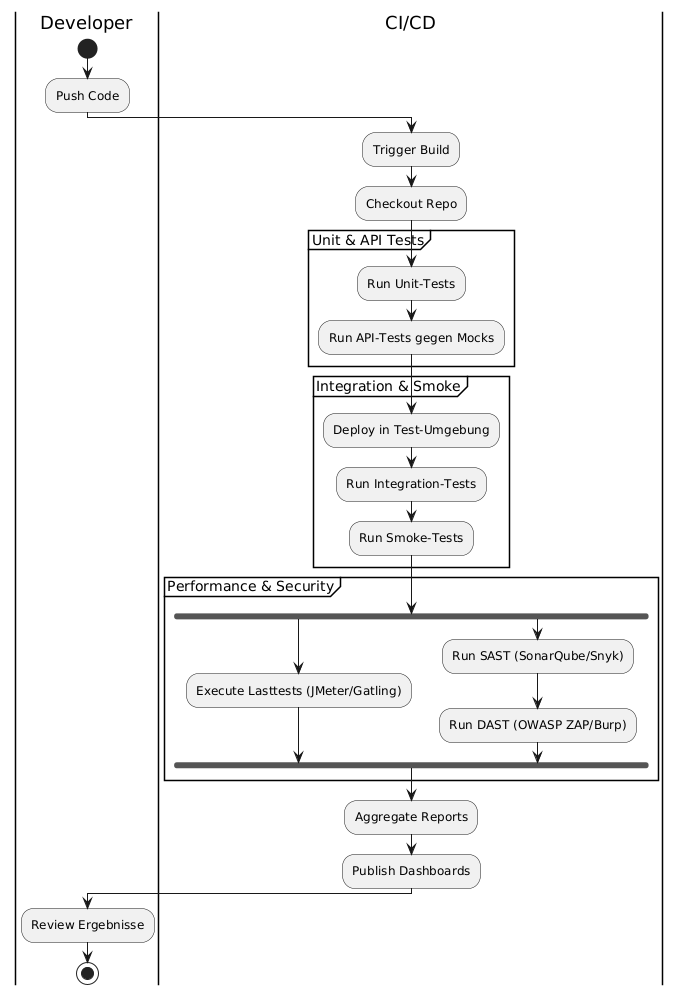
\includegraphics[width=0.9\textwidth]{fig/ablauf_pipeline.png}
    \caption{Ablaufflow: Continuous-Testing-Pipeline}
    \label{fig:flow}
\end{figure}

In Abbildung \ref{fig:flow} ist der Ablaufflow der Continuous-Testing-Pipeline dargestellt.
Diese Pipeline zeigt die verschiedenen Schritte, die in der Testumgebung durchgeführt werden,
nachfolgende eine kurze Beschreibung der einzelnen Schritte:

\begin{itemize}
    \item \textbf{Unit \& API Tests} laufen sofort gegen Mocks und Stubs.
    \item \textbf{Integration \& Smoke} werden in einer auf IaC bereitgestellten Testumgebung durchgeführt.
    \item \textbf{Performance \& Security} finden parallel in eigenen Phasen statt.
    \item Abschließend werden alle Reports zusammengeführt und im Dashboard veröffentlicht.
\end{itemize}  

\clearpage


\subsubsection{Prozessorientierte Testarchitektur für Foto-Webshop}
\begin{figure}[h!]
\centering
    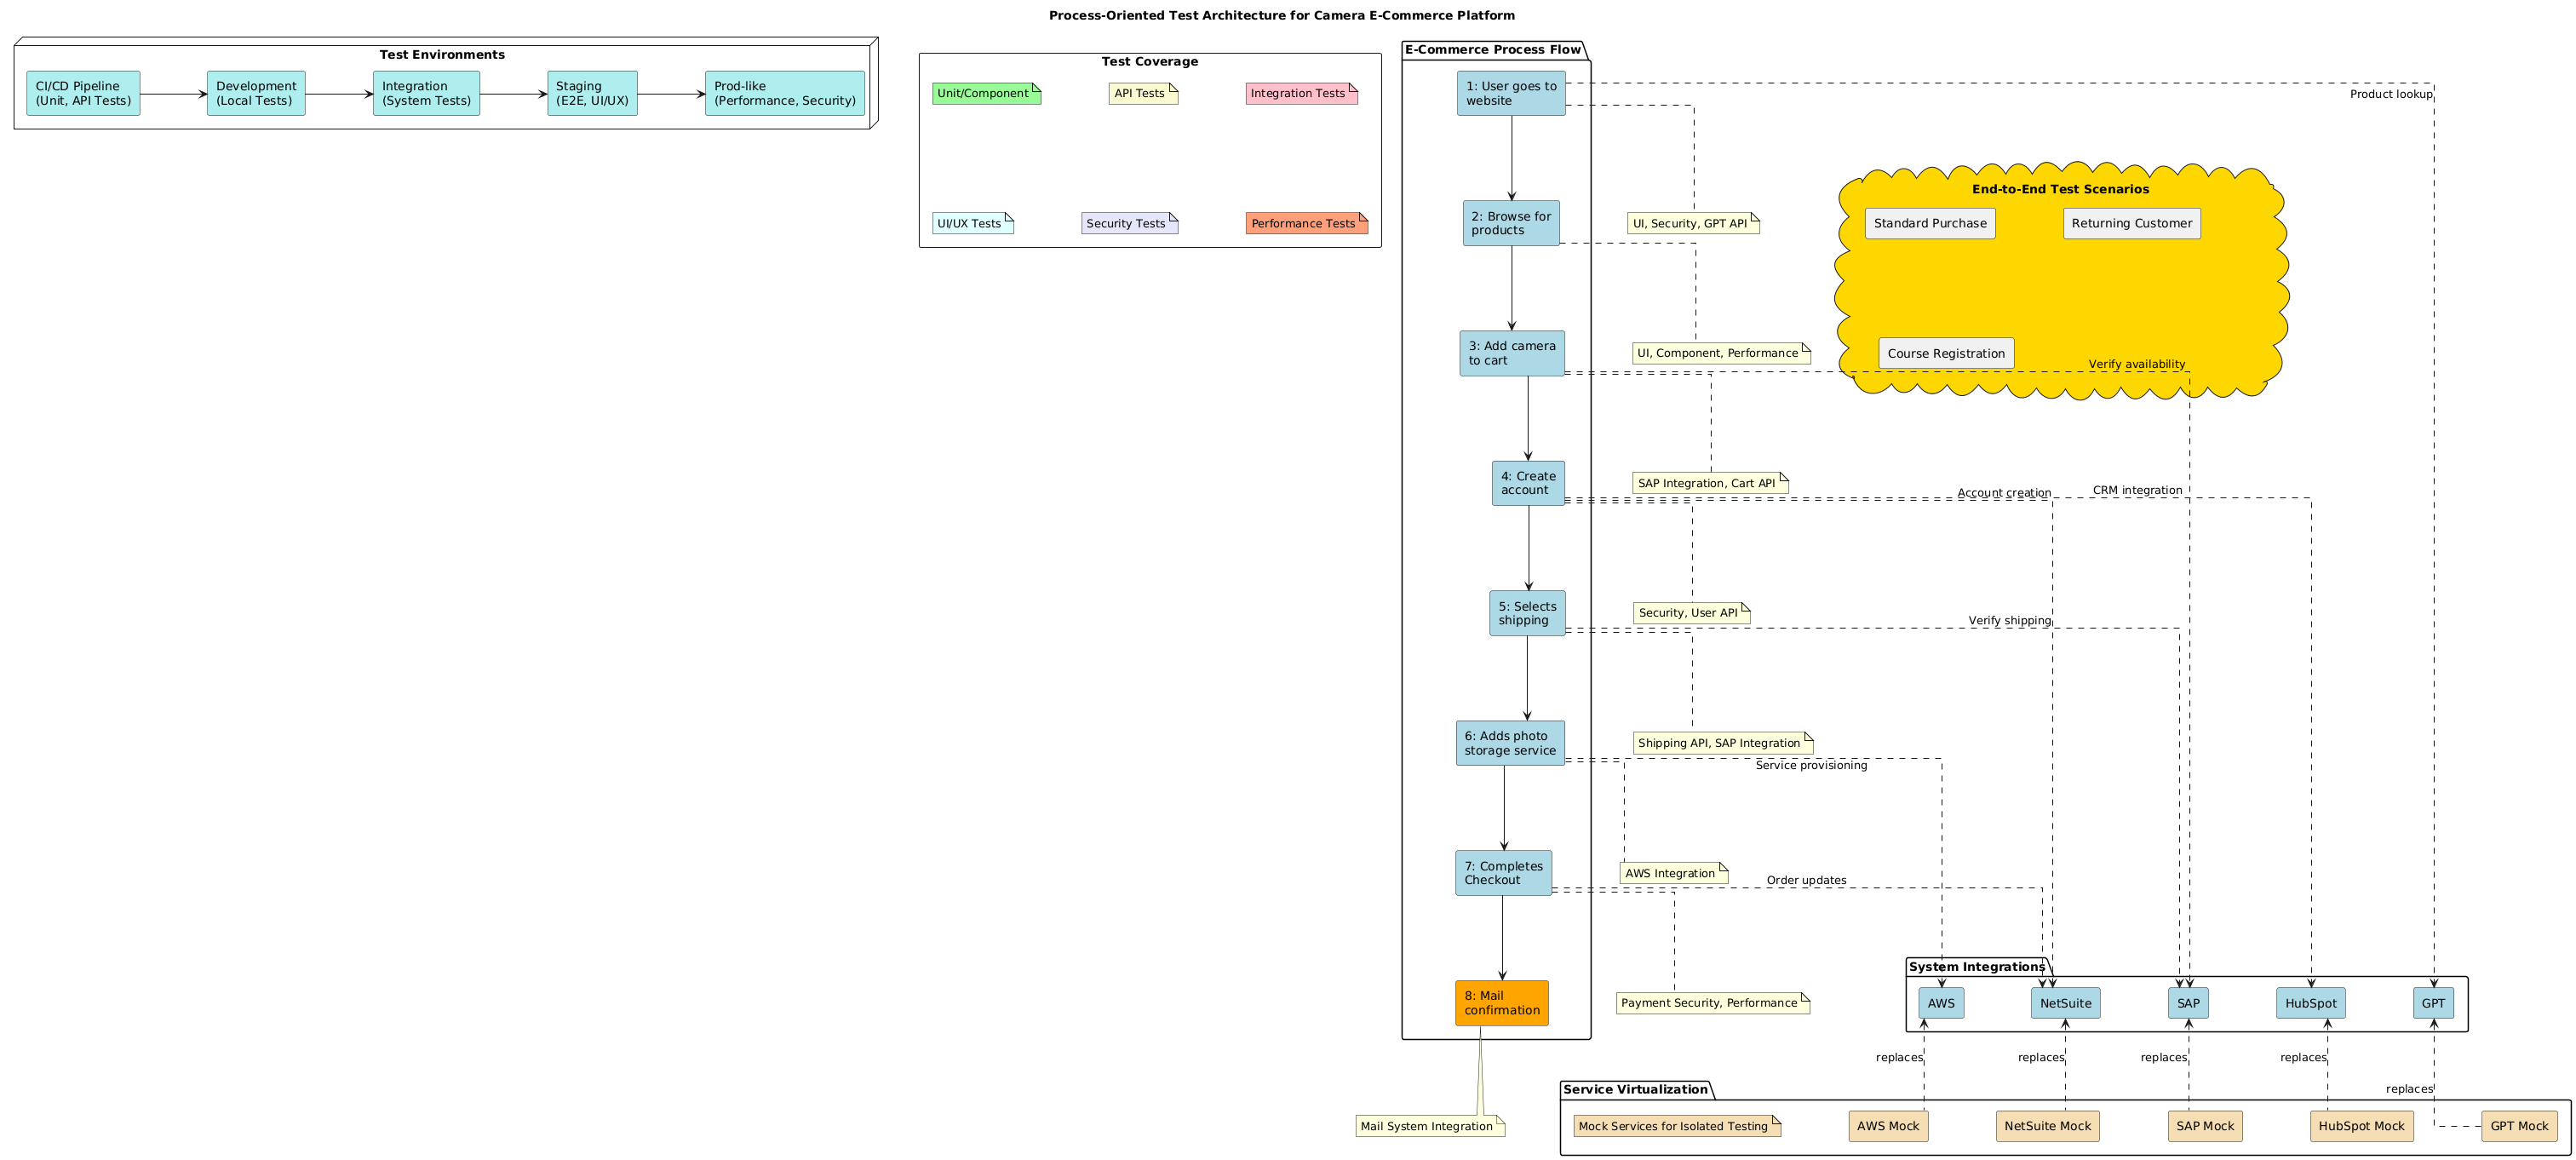
\includegraphics[width=1.1\textwidth]{fig/prozessschritte.png}
    \caption{Prozessorientierte Testarchitektur}
    \label{fig:flow2}
\end{figure}